%%%%%%%%%%%%%%%%%%%%%%%%%%%%%%%%%%%%%%
%option a4paper if needed
\documentclass[11pt,twocolumn,a4paper]{article}

%% Language and font encodings
\usepackage[protrusion=true,expansion=true]{microtype} % Better typography
\usepackage[english]{babel}
\usepackage[utf8x]{inputenc}
\usepackage[T1]{fontenc}
\usepackage[normalem]{ulem}
\usepackage{natbib}
\renewcommand{\refname}{\normalfont\selectfont\normalsize\bf References} 
\setlength{\bibsep}{0.0pt}
\usepackage[small]{caption}

%% Useful packages
\usepackage{amsmath}
\usepackage{graphicx}
\usepackage[colorinlistoftodos]{todonotes}
\usepackage[colorlinks=true, allcolors=blue]{hyperref}
\newcommand\blue{\bf\color{blue}}
\newcommand\HI{H\,{\small I}~}
\newcommand\spix{{\small SPINNAKER}}

% Margins
\topmargin=-0.40in
\evensidemargin=-0.38in
\oddsidemargin=-0.38in
\textwidth=7.0in
\textheight=9.9in
\headsep=0.25in 

  
\begin{document}


\title{SPINNAKER User Manual}
\author{Volker Heesen}
 
\maketitle


\begin{figure}
  \centering
  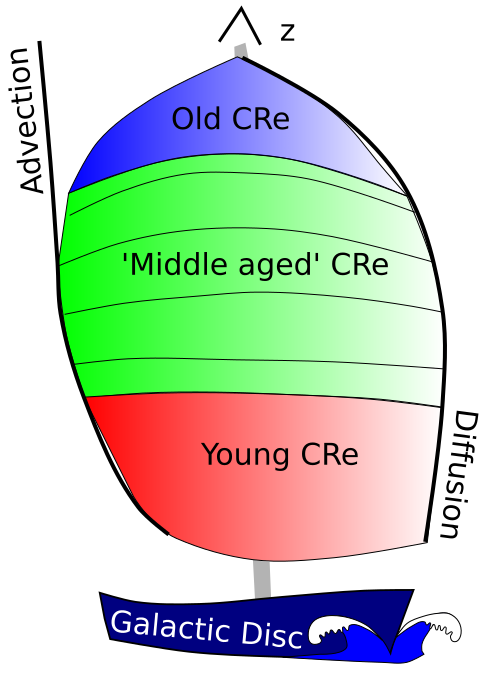
\includegraphics[width=0.5\textwidth]{Spinnaker_Logo}
\end{figure}



\noindent {\bf Summary.} This documents explains the usage of \spix, the Spectral INdex Numerical Analysis of K(c)osmic-ray Electron Radio-emission.

\section{Parameter file}
{\small SPINNAKER} is controlled using the `parameters' file of which I explain now the input parameters. I have divided the parameter file into several sections in order to make the process of filling them in a bit easier to oversee.\\

\subsection{Setup of the 2-dimensional grid}
\label{sec:setup_of_the_2D_grid}
\begin{itemize}
\item {\tt grid\_size}:  Number of data points in z-direction. I recommend using at least 100 with up to 400 possible.\\
\emph{Default: {\tt grid\_size = 200}}
\item {\tt nu\_channel}: Number of data points in frequency direction. As with {\tt grid\_size}, I recommend using at least 100 with up to 400 possible.\\
\emph{Default: {\tt nu\_channel = 200}}
\item {\tt grid\_delta}: This determines which data points are printed into the output files. The reason for this is that for numerical accuracy one needs more data points for the computation than are eventually compared with the observed data.\\
\emph{Default: {\tt grid\_delta = 10}}
\item {\tt z\_halo}: This is the physical size of the $z$-direction. E.g.\ choosing ${\tt z\_halo} = 10~\rm kpc$, will compute the CRE spectra between 0 and 10~kpc.
\item {\tt first\_data\_point\_at\_0kpc}: Set this parameter to 1, so that the first data point of the \emph{output files} is at 0~kpc. I included this parameter because using the program {\small STRIPS} by Rainer Beck will lead to vertical profiles that are symmetric around 0 but do not include 0 in the data. Then this parameter has to be set to $-1$. The output files are then beginning at $0.5\times grid\_delta$.\\
\emph{Default: {\tt first\_data\_point\_at\_0kpc = $\tt -1$}}
\item {\tt normalize\_intensities}: Setting this parameter to 1, means all intensities at the four observing frequencies are normalized to 1 at $z=0~\rm kpc$. This can be useful if one needs e.g.\ the second frequency $\nu_2$ for the intensity model. Usually this is not needed and if the parameter is set to $-1$, the intensities are all calculated according to their radio spectral indices.\\
\emph{Default: {\tt normalize\_intensities = $\tt -1$}}
\end{itemize}

\subsection{Output}
\begin{itemize}
\item {\tt nu\_1}: First output frequency in units of Hz. E.g. {\tt nu\_1 = 1.37e9} means $\nu_1=1.37\times 10^{9}~\rm Hz$.\\
\emph{Default: {\tt nu\_1 = $\tt 1.37e9$}}
\item {\tt nu\_2}: Second output frequency in units of Hz. E.g. {\tt nu\_2 = 4.86e9} means $\nu_2=4.86\times 10^{9}~\rm Hz$.\\
\emph{Default: {\tt nu\_2 = $\tt 4.86e9$}}
\item {\tt nu\_3}: Third output frequency in units of Hz. E.g. {\tt nu\_3 = 6.20e9} means $\nu_3=6.20\times 10^{9}~\rm Hz$.\\
\emph{Default: {\tt nu\_3 = $\tt 6.20e9$}}
\item {\tt nu\_4}: Fourth output frequency in units of Hz. E.g. {\tt nu\_4 = 8.40e9} means $\nu_4=8.40\times 10^{9}~\rm Hz$.\\
\emph{Default: {\tt nu\_4 = $\tt 8.40e9$}}
\item {\tt mode}: Use either pure advection ({\tt mode = 1}) or pure diffusion ({\tt mode = 2}).\\
\emph{Default: {\tt mode = 1}}
\item {\tt epsilon}: If {\tt epsilon = 1}, synchrotron emissivities instead of intensities are calculated. In order to do this, the radius $r$ of the outflow needs to be provided as part of the magnetic field model (see below).
\end{itemize}


\begin{figure*}
  \centering
  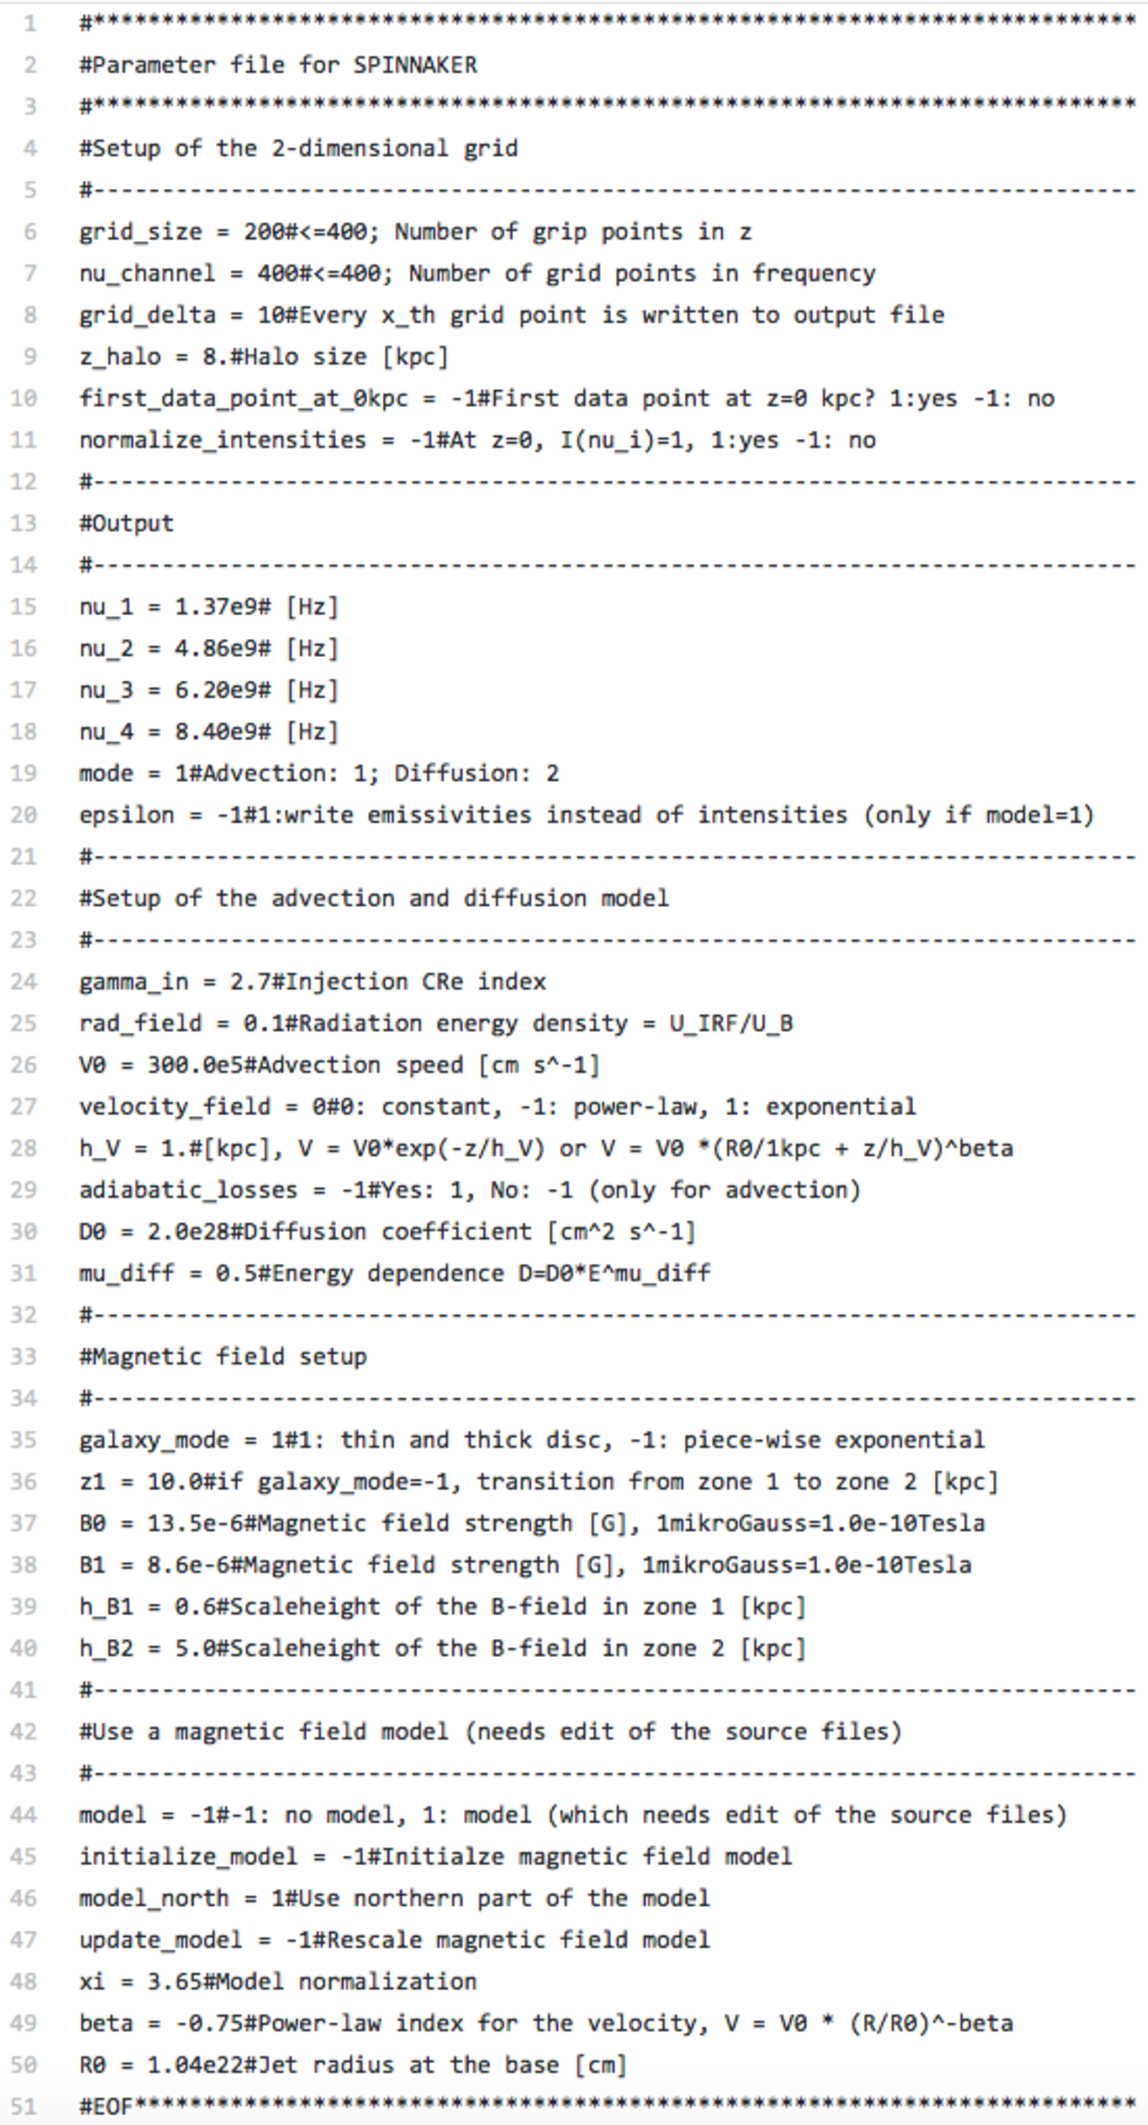
\includegraphics[width=0.7\textwidth]{parameters}
  \caption{Parameter file with the inputs for \spix.}
\label{fig:parameters}
\end{figure*}

\subsection{Setup of the advection and diffusion model}
\begin{itemize}
\item {\tt gamma\_in}: This is the CRE injection spectral index. In \spix, this is not equivalent to the theoretical injection spectral index of young CREs in supernova remnants which is quite flat with $\gamma_{\rm inj}=2$ where $N(E,z=0)\propto E^{-\gamma_{\rm inj}}$. Instead in \spix, this parameter is free and has to be determined from the fitting.\\
\emph{Default: {\tt gamma\_in = $\tt 2.7$}}
\item {\tt rad\_field}: This parameter determines the ratio of the radiation energy density of the interstellar radiation field (IRF), excluding the contribution from the cosmic microwave background, to the magnetic energy density $U_{\rm IRF}/U_{\rm B}$.\\
\emph{Default: {\tt rad\_field = $\tt 0.1$}}
\item {\tt V0}: The advection speed in the galactic midplane ($z=0~\rm kpc$) in units of $\rm cm\,s^{-1}$. E.g. {\tt V0 = 300.0e5} means $V_0 = 300~\rm km\,s^{-1}$.\\
\emph{Default: {\tt V0 = 300.0e5}}
\item {\tt velocity\_field}: This parameter determines the shape of the velocity field. For {\tt velocity\_field = 0}, the advection speed is constant everywhere. For {\tt velocity\_field = -1}, the advection speed follows a power law $V(z)=V_0\cdot (r/r_0)^{\beta}$, where $r$ is the radius of the outflow and $\beta$ is the velocity acceleration/decceleration parameter. This option is only possible if a magnetic field model (see below) is given. For {\tt velocity\_field = 1}, the advection speed changes exponentially as $V(z) = V_0\cdot \exp(-z/h_{\rm V}$.\\
\emph{Default: {\tt velocity\_field = 0}}
\item {\tt adiabatic\_losses}: Setting {\tt adiabatic\_losses = 1}, switches additional adiabatic losses on which are important for an accelerating wind (advection).\\
\emph{Default:} {\tt adiabatic\_losses = $\tt -1$}
\item {\tt D0}: Diffusion coefficient at a CRE energy of 1~GeV in units of $\rm cm^{2}\,s^{-1}$. E.g.\ setting {\tt D0 = 2.0e28} means $D_0=2.0\times 10^{28}~\rm cm^2\,s^{-1}$.\\
\emph{Default:} {\tt D0 = 2.0e28}
\item {\tt mu\_diff}: Energy dependence of the diffusion coefficient with $D=D_0\cdot (E/1~{\rm GeV})^\mu$.\\
\emph{Default:} \emph{{\tt mu\_diff = $\tt 0.5$}}
\end{itemize}

\subsection{Magnetic field setup}
\label{sec:magnetic_field_setup}
\begin{itemize}
\item {\tt galaxy\_mode}: If {\tt galaxy\_mode = 1}, then the magnetic field is a superposition of the thin and the thick disc with $B(z) = B_1 \cdot \exp(-z/h_{\rm B1}) + (B_0-B_1)\cdot \exp(-z/h_{\rm B2})$.  If {\tt galaxy\_mode = $\tt -1$}, then magnetic field is piece-wise exponential with $B(z) = B_0\cdot \exp(-z/h_{\rm B1})$ for $z\leq z_1$ and $B(z) = B_0\cdot \exp(-z_1/h_{\rm B1})\cdot\exp(-z/h_{\rm B2})$ for $z>z_1$. The latter mode is possibly more suitable for the lobes of a radio galaxy.\\
\emph{Default: {\tt galaxy\_mode = 1}}
\item {\tt z1}: If {\tt galaxy\_mode = $\tt -1$}, then this parameter, $z_1$, is used for the transition of the piece-wise exponential function. This parameter is also useful if one wants to have only a thin or a thick disc. Setting $\tt z1$ larger than $\tt z_halo$ in conjunction with {\tt galaxy\_mode = $\tt -1$} will do just that. The units of $\tt z1$ are in kpc.\\
\emph{Default: {\tt z1 = 10}}
\item {\tt B0}: Strength of the magnetic field in the galactic midplane in units of Gauss ($= 10^{-4}~\rm Tesla$). E.g.\ setting {\tt B0 = $\tt 13.5e-6$} means $B_0 = 13.5~\mu\rm G$.
\\
\emph{Default:} {\tt B0 = $\tt 13.5e-6$}
\item {\tt B1}: If {\tt galaxy\_mode = 1}, then this is the strength of the magnetic field of the thin disc component in units of Gauss ($= 10^{-4}~\rm Tesla$). E.g.\ setting {\tt B1 = $\tt 8.6e-6$} means $B_1 = 8.6~\mu\rm G$.\\
\emph{Default:} {\tt B1 = $\tt 8.6e-6$}\\
\item {\tt h\_B1}: Scale height of the magnetic field of the thin disc component (if {\tt galaxy\_mode = 1}) or for $z\leq z_1$ (if {\tt galaxy\_mode = $\tt -1$}). The units of {\tt h\_B1} are in kpc.\\
\emph{Default:} {\tt h\_B1 = $\tt 0.6$}
\item Scale height of the magnetic field of the thick disc component (if {\tt galaxy\_mode = 1}) or for $z> z_1$ (if {\tt galaxy\_mode = $\tt -1$}). The units of {\tt h\_B2} are in kpc.\\
\emph{Default:} {\tt h\_B2 = $\tt 5.0$}
\end{itemize}
\begin{figure*}
  \centering
  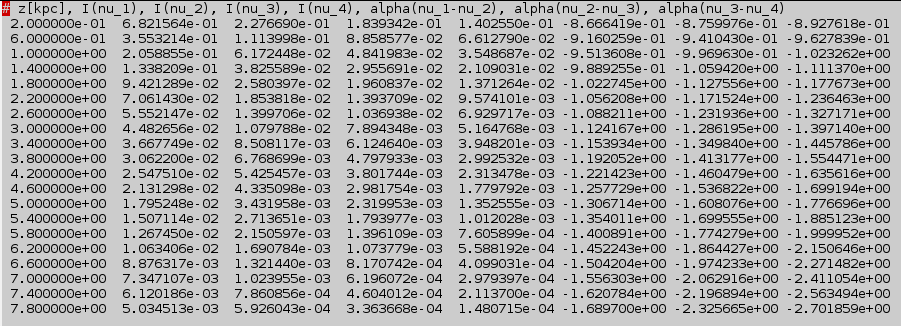
\includegraphics[width=1.0\textwidth]{int}
  \caption{Output file {\tt int.dat} as obtained with the default parameters.}
\label{fig:int}
\end{figure*}
{\bf Magnetic field model}\\
This section can be used in order to specify a magnetic field model for every data point in $z$-direction, rather than using exponential functions. Thus far, this requires the editing of the code source files and a recompilation.
\begin{itemize}
\item {\tt model}: The option to use a magnetic field model can be switched on setting {\tt model = 1}. Setting {\tt model = $\tt -1$}, then no model is used.\\
\emph{Default:} {\tt model = $\tt -1$}
\item {\tt initialize\_model}: If {\tt initialize\_model = 1}, then the magnetic field model is initialized with the analytic (exponential) magnetic field model from the previous section. This has to be done first, with the magnetic field adjusted iteratively in the following steps.
\item {\tt model\_north}: For a galaxy or radio galaxy, two haloes/lobes can be analysed. If {\tt model\_north = 1}, then the model for the northern halo is used.  If {\tt model\_north = $\tt -1$}, the model for the southern halo is used.\\
\emph{Default:} {\tt model\_north = 1}
\item {\tt update\_model}: If {\tt update\_model = 1}, the magnetic field model is updated using the provided intensities. This should be done until the fit converges.\\
\emph{Default:} {\tt update\_model = $\tt -1$}
\item {\tt xi}: This is the model normalization parameter $\xi$. The parameter has to be adjusted in such a way that the magnetic field strength at $z=0~\rm kpc$ is unchanged and still $B_0$. If the model magnetic field strength drifts to higher values than $B_0$, then $\tt xi$ has to be higher. If the model magnetic field strength drifts to lower values than $B_0$, then $\tt xi$ has to be lower.
\item {\tt beta}: This is the velocity acceleration/deceleration parameter that can be used if a magnetic field model with radius values is provided. For {\tt velocity\_field = -1}, the advection speed follows a power law $V(z)=V_0\cdot (r/r_0)^{\beta}$, where $r$ is the radius of the outflow and $\beta$ is the velocity acceleration/decceleration parameter.\\
emph{Default:} {\tt beta = $\tt -0.75$}
\item {\tt R0}: Radius at the base of the outflow or in the galactic midplane ($Z=0~\rm kpc$) in units of cm. E.g.\ setting {\tt R0 = $\tt 1.04e22$} means $r_0 = 1.04\times 10^{22}~\rm cm$.\\
\emph{Default}: {\tt R0 = $\tt 1.04e22$}
\end{itemize}


\section{Output files}
In this section, I present the use of the various output files which are produced by \spix. Running \spix with the default parameters will result in the output files that I discuss in what follows.

\subsection {Non-thermal intensities and spectral indices}
The output file is {\tt int.dat}, see Fig.~\ref{fig:int}, and has the following columns:
\begin{itemize}
\item Column 1 / {\tt z[kpc]}: This is the distance to the galactic midplane in units of kpc.
\item Column 2 / {\tt I(nu\_1)}: This is the non-thermal (synchrotron) intensity as calculated at the observing frequency $\nu_1$.
\item Column 3 / {\tt I(nu\_2)}: This is the non-thermal (synchrotron) intensity as calculated at the observing frequency $\nu_2$.
\item Column 4 / {\tt I(nu\_3)}: This is the non-thermal (synchrotron) intensity as calculated at the observing frequency $\nu_3$.
\item Column 5 / {\tt I(nu\_4)}: This is the non-thermal (synchrotron) intensity as calculated at the observing frequency $\nu_4$.
\item Column 6 / {\tt alpha(nu\_1-nu\_2)}: This is the non-thermal radio spectral index between frequencies $\nu_1$ and $\nu_2$.
\item Column 7 / {\tt alpha(nu\_2-nu\_3)}: This is the non-thermal radio spectral index between frequencies $\nu_2$ and $\nu_3$.
\item Column 8 / {\tt alpha(nu\_3-nu\_4)}: This is the non-thermal radio spectral index between frequencies $\nu_3$ and $\nu_4$.
\end{itemize}

This output file is the most important one and allows the fitting of the non-thermal model intensities and spectral indices to the observed data. 

\subsection{Magnetic field strength and advection velocity}
The output file is {\tt b.dat}, see Fig.~\ref{fig:b}.
\begin{itemize}
\item Column 1 / {\tt z[kpc]}: This is the distance to the galactic midplane in units of kpc.
\item Column 2 / {\tt B [G]}: This is the magnetic field strength in units of Gauss.
\item Column 3 / {\tt V [cm~s\^-1]}: This is the advection speed in units of $\rm cm\,s^{-1}$.
\end{itemize}

\subsection{CRE number densities}
The output file is {\tt ne.dat}.
\begin{itemize}
\item Column 1 / {\tt z[kpc]}: This is the distance to the galactic midplane in units of kpc.
\item Column 2 / {\tt N (nu\_1)}: CRE number density at the critical frequency of $\nu_1$ for the magnetic field strength in the galactic midplane .
\item Column 3 / {\tt N (nu\_1\_crit)}: CRE number density at the critical frequency of $\nu_1$ for the magnetic field strength $B(z)$.
\item Column 4 / {\tt N (nu\_2\_crit)}: CRE number density at the critical frequency of $\nu_2$ for the magnetic field strength $B(z)$.
\end{itemize}

\begin{figure}
  \centering
  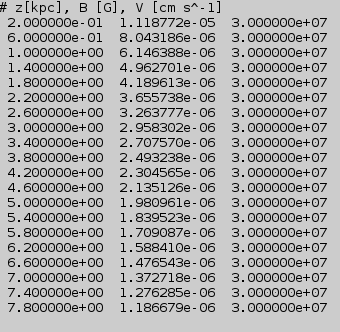
\includegraphics[width=0.5\textwidth]{b}
  \caption{Output file {\tt b.dat} as obtained with the default parameters.}
\label{fig:b}
\end{figure}


\begin{figure*}
  \centering
  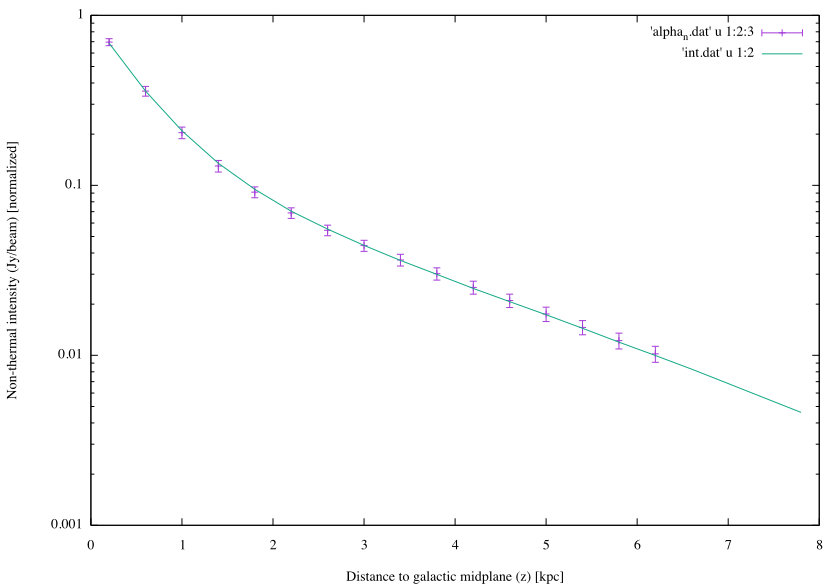
\includegraphics[width=0.9\textwidth]{intensity_profile}
  \caption{Non-thermal model intensities at $1.37~\rm GHz$ in the northern halo of NGC~4631 as data points with error bars. The line shows the model intensities as calculated with \spix.}
\label{fig:intensity_profile}
\end{figure*}

\subsection{Non-thermal spectrum}
The output file is {\tt spec.dat}. This output requires the editing of the source files and re-compilation in order to define the 6 different $z$-values at which the spectrum is read out.
\begin{itemize}
\item Column 1 / {\tt nu[Hz]}: Observing frequency in units of Hz.
\item Column 2 / {\tt I(z\_1)}: Non-thermal intensity at the position {\tt z\_1}  (note that this position is not identical to $z_1$ from the magnetic field setup in Section~\ref{sec:magnetic_field_setup}).
\item Column 3 / {\tt I(z\_2)}: Non-thermal intensity at the position {\tt z\_2} .
\item Column 4 / {\tt I(z\_3)}: Non-thermal intensity at the position {\tt z\_3}.
\item Column 5 / {\tt I(z\_4)}: Non-thermal intensity at the position {\tt z\_4}.
\item Column 6 / {\tt I(z\_5)}: Non-thermal intensity at the position {\tt z\_5}.
\item Column 7 / {\tt I(z\_6)}: Non-thermal intensity at the position {\tt z\_6}.
\end{itemize}


\begin{figure*}
  \centering
  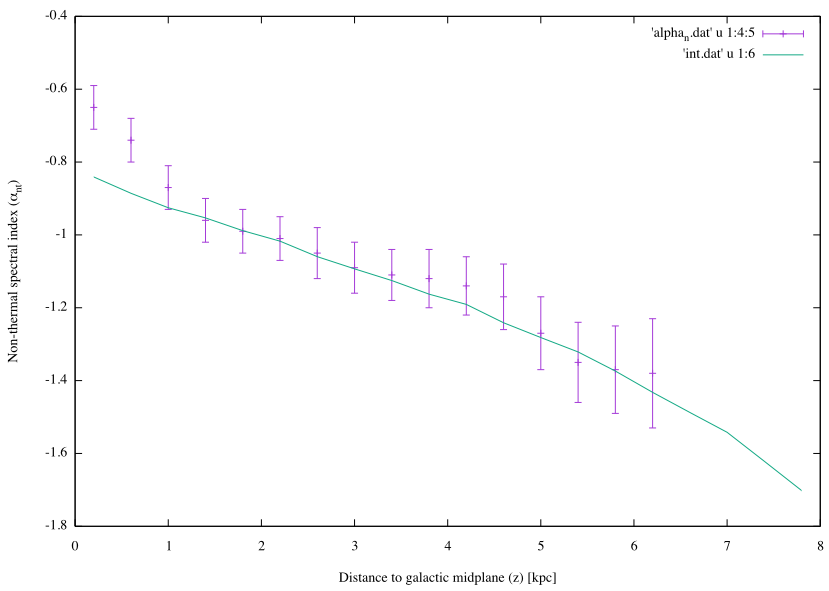
\includegraphics[width=0.85\textwidth]{alpha_profile}
  \caption{Non-thermal radio spectral index between $1.37$ and $4.86~\rm GHz$ in the northern halo of NGC~4631 as data points with error bars. The line shows the model spectral index as found in Column 6 of the file {\tt int.dat}.}
\label{fig:alpha_profile}
\end{figure*}


\subsection{CRE spectrum}
The output file is {\tt ne\_spec.dat}. As with {\tt spec.dat}, this output requires the editing of the source files and re-compilation in order to define the 6 different $z$-values at which the spectrum is read out.
\begin{itemize}
\item Column 1 / {\tt nu[Hz]}: Observing frequency in units of Hz.
\item Column 2 / {\tt I(z\_1)}: CRE number density at the position {\tt z\_1}  (note that this position is not identical to $z_1$ from the magnetic field setup in Section~\ref{sec:magnetic_field_setup}).
\item Column 3 / {\tt I(z\_2)}: CRE number density at the position {\tt z\_2}.
\item Column 4 / {\tt I(z\_3)}: CRE number density at the position {\tt z\_3}.
\item Column 5 / {\tt I(z\_4)}: CRE number density at the position {\tt z\_4}.
\item Column 6 / {\tt I(z\_5)}: CRE number density at the position {\tt z\_5}.
\item Column 7 / {\tt I(z\_6)}: CRE number density at the position {\tt z\_6}.
\end{itemize}

\section{NGC~4631 as an example}
In this section, I present the example results for the northern halo of NGC~4631 for which the default parameters have been already fitted. In Fig.~\ref{fig:intensity_profile}, I show the non-thermal model intensities in the northern halo of NGC~4631 as data points with error bars. These model intensities have been obtained by fitting two-component exponential functions to the vertical non-thermal intensity profile. The line represents the non-thermal intensities at $\nu=1.37~\rm GHz$ as calculated with \spix, taking the data from Column 2 in {\tt int.dat}. In the first step of fitting \spix to data, one has to adjust the magnetic field setup so that the intensities are fitted well.

In Fig.~\ref{fig:alpha_profile}, the corresponding non-thermal radio spectral index profile between $1.37$ and $4.86~\rm GHz$ is shown. Again, the lines shows the \spix model profile, taking Column 6 of the file {\tt int.dat}. In the second step of fitting \spix to the data, the injection spectral index and the advection has to be varied so that the spectral indices are fitted well. Obviously, changing the advection speed changes the resulting model intensities profiles, so it takes a bit of trying in order to be able to fit the intensities and the spectral indices \emph{simulataneously}.

During the fitting and as an end result, one can plot the \spix model magnetic field strength, which is shown in Fig.~\ref{fig:b_profile}. This is simply plotting Column 2 of the file {\tt b.dat}.




\begin{figure*}
  \centering
  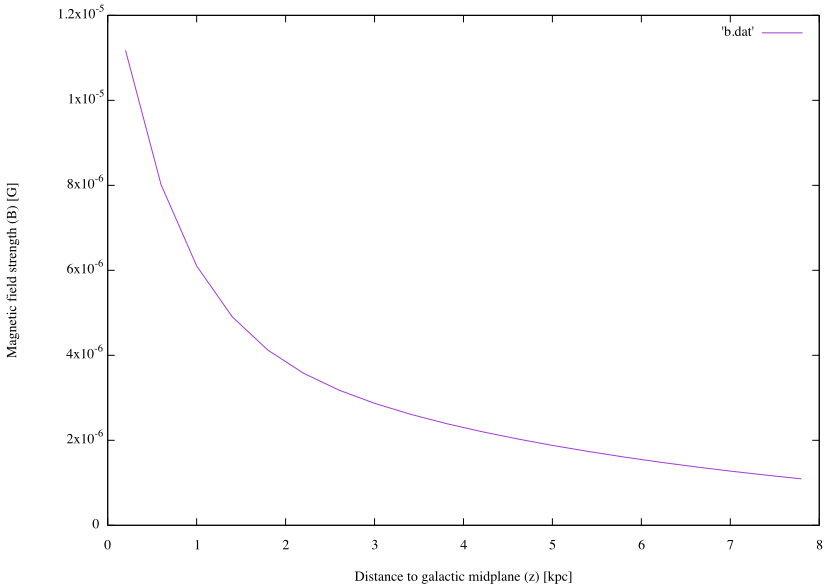
\includegraphics[width=0.95\textwidth]{b_profile}
  \caption{Model magnetic field strength calculated with \spix in the northern halo of NGC~4631. The data are taken from Column 2 of the file {\tt b.dat}.}
\label{fig:b_profile}
\end{figure*}


\begin{thebibliography}{99}
\bibitem[Heesen et~al\mbox{.}(2016)]{heesen_16a} Heesen, V. et al.\ 2016,
  MNRAS, 458, 332
\end{thebibliography}

\end{document}

